\section{Framework}
\label{Framework}
\begin{figure}[!t]
\centering
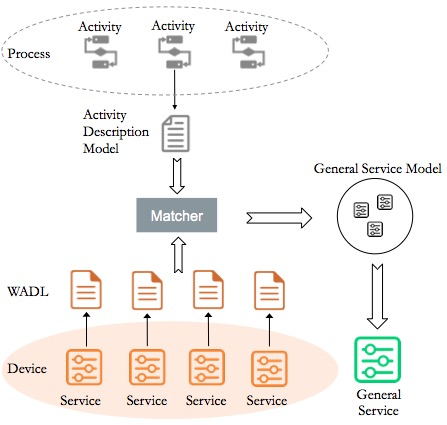
\includegraphics[width=1.0\linewidth]{./graph/framework}
% where an .eps filename suffix will be assumed under latex, 
% and a .pdf suffix will be assumed for pdflatex; or what has been declared
%via \DeclareGraphicsExtensions.
\caption{Overall architecture for the framework.}
\label{fig_framework}
\end{figure}
The overall architecture of our framework is shown in Fig.~\ref{fig_framework}. In a business process, each activity is bound to an activity description model. The model is defined in a XML structure by RDF, which is a recommended semantic modeling metadata. The model provides ontological annotations for the binding activity abouts it's functionalities and messages. In order to reduce extra work for modeling, an Eclipse plugin is offered to help users to construct the models more effectively after the process is  defined. 

The matcher is the central component. Once the device envrionment is changed, users can upload the WADL description of the services of the new device and the activity description model to the matcher. A semantic-based matching mechanism is executed to find suitable service composition strategy, and the matching result will be presented in a general service model. 

The general service model is consist of two part: (1) description of the general service, including resource path, request method, request and response parameters, and (2)actual service instances to composite and parameters mappings. On the basis of the model, a general service can be automatically generated. For the invoker of the general service, the service provides a device-independent request interface, which means that the invoker is able to call the general services from different devices that have the same capabilities of the process activity and don't need to modify the HTTP request at all. 